\chapter{Fundamento Teórico}

La sección de canal van a dar pie a los time interleavers y esas cosas, no? O sea, hablar de fading tanto en frecuencia y tiempo y cómo contrarrestarlo?
Yo pondría la parte de DFT, FFT y convolución circular dentro de OFDM. En FFT van a hablar del algoritmo? Me parece medio al santo botón.
En la parte de códigos les faltó hablar de convolucionales.


\section{Modelado del canal}
	\subsection{Canales Continuos}
	\subsection{Canales Discretos}
	\subsection{Las no idealidades del Canal}
No idealidades del canal inalámbrico móvil.

\section{Estrategias para mitigar los efectos del canal}

	\subsection{C\'odigos de detecci\'on y correci\'on de errores}

La comunicación entre emisor y receptor puede modelarse mediante el proceso de la Figura \ref{diagrama_codificacion}. La situación es la siguiente, una fuente emisora envía mensajes $m$ (palabras fuente) al receptor a través de un canal de comunicación. El mensaje debe ser traducido a algún mensaje que el canal esté capacitado para enviar, estos mensajes se conocen como palabras código.

\begin{figure}
\centering
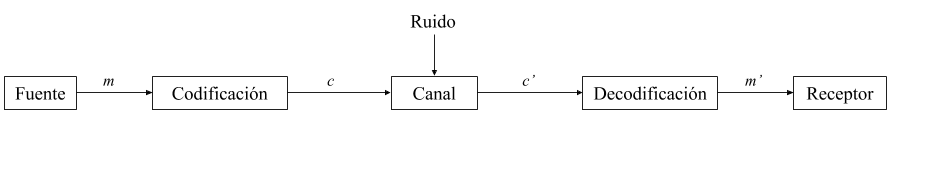
\includegraphics[scale=0.45]{figuras/cap02/diagrama_codificacion}
\caption{\label{diagrama_codificacion} Esquema básico de codificación de canal.}
\end{figure}

Al otro lado del canal llega un mensaje codificado $c'$, el cual seguramente sea erróneo, pues en todo proceso real de comunicación existe ruido e imperfecciones en los canales. El mensaje es decodificado en una palabra $m'$, y generalmente $m' \neq m$.

Se desea que el receptor sea capaz de darse cuenta si el mensaje $m'$ es realmente lo que se transmitió del otro lado, y más aún, poder corregirlo. 

La Teoría de Códigos es un campo de la matemática aplicada que busca resolver los problemas de las etapas de codificación-decodificación y corrección, y que presenta su propia complejidad.

La transmisión inalámbrica de una señal la expone a diversas fuentes de ruido, con lo cual los tipos de errores generados pueden ser muy variados. Por ejemplo los errores en ráfaga, en los que un conjunto de bits consecutivos se ven alterados, son muy comunes en las comunicaciones inalámbricas. También podría suceder que el canal radioeléctrico presente distorsión en algunas portadoras en particular.

El estándar ISDB-T hace uso de distintas técnicas modernas para la protección de los datos en transmisión. De hecho para proteger los datos en los ejemplos mencionados el estándar utiliza la \textit{dispersión de energía} y el  \textit{entrelazamiento frecuencial}. Para la comprensión del estándar y el desarrollo de \textit{gr-isdbt-tx}, es importante conocer el funcionamiento de estas técnicas. Profundizar en estos temas escapa los objetivos de este trabajo, por lo cual los detalles técnicos se pueden encontrar en las bibliografías mencionadas.

Para asegurarse que el receptor pueda llevar a cabo satisfactoriamente la demodulación y decodificación en una transmisión jerárquica, en la cual se utilizan múltiples parámetros de transmisión, se utiliza una señal denominada Transmission and Multiplexing Configuration Control (TMCC).

Como se verá en el Capítulo XX, la TMCC junto con otras señales piloto y las señales correspondientes a la transmisión de los datos útiles, conforman el cuadro OFDM.

Al tratarse de una señal que contiene información crítica sobre la transmisión se la debe proteger fuertemente frente a los distintos tipos de errores que podría sufrir durante su transmisión.

En particular ISDB-T establece que para la TMCC se debe utilizar el código acortado (200,118) del \textit{difference-set cyclic code} (273,191) como código corrector de errores.

\subsection{Códigos Cíclicos}
El conjunto $GF(2) \triangleq \{0,1\}$, con las operaciones de suma $" + "$ y producto $" \times "$ usuales módulo 2, cumple con la propiedad de que cualquier elemento de $GF(2)$ distinto de cero tiene inverso. Esta propiedad se cumple trivialmente en este conjunto y es la condición necesaria para que $GF(2)$ sea un \textit{Campo de Galois}. Es común encontrar que a este campo también se lo llame \textit{campo binario} y se lo denote como $\mathbb {F}_2$.
Las operaciones de suma y producto definidas en $GF(2)$ son asociativas, conmutativas y distributivas, y llevan elementos de $GF(2)$ en elementos de $GF(2)$. Por esto $GF(2)$ también es un \textit{anillo}. 
El conjunto de todos los polinomios con coeficientes en $GF(2)$ con las operaciones usuales de suma y producto forman un \textit{anillo de polinomios} en $GF(2)$ y se denota como $GF(2)[x]$. Por ejemplo $g(x) = x^3 + x + 1$ es un elemento de $GF(2)[x]$.

Sea $\textbf{c} = (c_0, c_1, ..., c_{n-1}) \in GF(2)$, con $GF(2)$ tal como se describió anteriormente. Un código $\mathcal{C}$ de bloque $(n, k)$ se dice que es un \textit{código cíclico} si para cada vector $\textbf{c} = (c_0, c_1, ..., c_{n-1}) \in \mathcal{C}$ cualquier rotación circular a la derecha de $C$ también pertenece a $\mathcal{C}$, es decir $(c_{n-1}, c_0, c_1, ..., c_{n-2}) \in \mathcal{C}$.
Los códigos de bloque se caracterizan por codificar mensajes de longitud fija $k$ en \textit{codewords} de longitud fija $n$, con lo cual el tamaño del mensaje original se incrementa en $n-k$.
Cada \textit{codeword} del código $\mathcal{C}$ puede ser representada en una forma polinomial de la siguiente manera:

\begin{equation}
c(x) = \sum_{i = 0}^{n-1}c_i x^i
\end{equation}

A continuación se enumera una serie de propiedades de los códigos cíclicos, en \cite{moon2005error} se puede encontrar una demostración detallada de cada una de ellas.

\begin{itemize}
\item{Un código cíclico es un código lineal de bloque}
\item{Cada \textit{codeword} se corresponde con un polinomio}
\item{Los polinomios del código forman un \textit{ideal} en $GF(2)[x]/(x^n-1)$}
\item{Para un código cíclico existe un generador $g(x)$ que es divisor de $x^n-1$ y que puede generar todos las \textit{codewords} $c(x)=m(x)g(x)$}
\end{itemize}

Se puede probar que esto implica la existencia de una \textit{matriz de chequeo de paridad} $\mathbb{H} \in \mathcal{M}_{(n-k)\times n}$ tal que para toda \textit{codeword} \textbf{c} de $\mathcal{C}$ se cumple $\textbf{c} \mathbb{H} ^T = \textbf{0}$.


El proceso de codificación se realiza de la siguiente manera, primero se construye el polinomio $x^{n-k}m(x)$ de grado $n$. Luego se divide entre el polinomio generador $g(x)$ y el resto de esa división es el polinomio de paridad $d(x)$ que se le agregará al mensaje:

\begin{equation}
x^{n-k}m(x) - q(x)g(x) = d(x)
\end{equation}

La \textit{codeword} se forma de la siguiente manera:

\begin{equation}
c(x) = x^{n-k}m(x)-d(x) = q(x)g(x)
\end{equation}

Como se trata de un múltiplo de $g(x)$, entonces efectivamente es una \textit{codeword} válida. La representación vectorial de la \textit{codeword} queda de la siguiente manera:

\begin{equation}
\textbf{c} = (-d_0, -d_1, ..., -d_{n-k-1}, m_0, m_1, ..., m_{k-1})
\end{equation}

En una situación en la que se recibe una palabra $\textbf{r}$ cuyo mensaje es $\textbf{m}$  y sus bits de paridad son $\textbf{d}$, el procedimiento para detectar si hubo error es codificar el mensaje $\textbf{m}$ que se recibió con el mismo codificador utilizado por el transmisor (ambas partes deben conocer el polinomio generador), y luego comparar el $\textbf{d'}$ obtenido con el $\textbf{d}$ recibido. Si ambos difieren entonces hubo error. 
Por ejemplo, para un código cíclico (7, 4) con polinomio generador $g(x) = x^3 + x + 1$ se desea codificar el mensaje 1001. Los mensajes codificados tendran $n-k = 7 - 4 = 3$ bits de paridad. El mensaje en su forma polinomial queda $m(x) = 1 + x^3$.
Los bits de paridad se obtienen calculando el resto de la division $x^{(7-4)}m(x)/g(x)$, los coeficientes de ese resto seran los bits de la paridad buscada. Operando se llega a que la paridad es 011 y el mensaje codificado queda 0111001.

	
	
	\subsection{C\'odigos BCH}
	\subsection{C\'odigos de Reed-Solomon}
	\subsection{Entrelazamiento de datos}

\section{Modulación OFDM}

	\subsection{Fundamentos}
		\subsubsection{Transformada de Fourier}
		\subsubsection{Convoluci\'on circular}
		\subsubsection{Esquema b\'asico}
	
	\subsection{Continuos}

	\subsection{Discretos}

\section{El estandard MPEG-4}
	\subsection{Generalidades}
	\subsection{Transport Stream Packet}
	\subsection{Tablas PAT}
	\subsection{Tablas PMT}

